\documentclass[11pt]{article}
\usepackage{fontspec}
\setmainfont{DejaVu Serif}
\setsansfont{DejaVu Sans}
\usepackage{polyglossia}\setmainlanguage{greek}\setotherlanguage{english}
\tolerance=2500\emergencystretch=3em
\usepackage{amsmath,amssymb}
\usepackage{geometry}\geometry{margin=2.4cm}
\usepackage{xcolor}\usepackage{graphicx}\usepackage{enumitem}\usepackage{booktabs}
\usepackage{caption}\captionsetup{font=small,labelfont=bf}
\usepackage[hidelinks]{hyperref}
\graphicspath{{figures/}}

\definecolor{ink}{HTML}{16212e}\definecolor{accent}{HTML}{1f5fa8}\definecolor{soft}{HTML}{eef3fb}
\definecolor{warn}{HTML}{a8341f}\definecolor{good}{HTML}{1f7a44}\color{ink}
\newcommand{\key}[1]{\par\medskip\noindent\colorbox{soft}{\parbox{\dimexpr\linewidth-2\fboxsep}{\textcolor{accent}{\textbf{Κλειδί:}}\ #1}}\par\medskip}
\newcommand{\ex}[1]{\par\smallskip\noindent\textbf{\textcolor{accent}{Παράδειγμα.}}\ #1\par\smallskip}
\newcommand{\warnb}[1]{\par\medskip\noindent\colorbox{soft}{\parbox{\dimexpr\linewidth-2\fboxsep}{\textcolor{warn}{\textbf{Προσοχή:}}\ #1}}\par\medskip}
\setlength{\parskip}{0.5em}\setlength{\parindent}{0pt}
\usepackage{titlesec}
\titleformat{\section}{\large\bfseries\color{accent}}{\thesection.}{0.5em}{}
\titleformat{\subsection}{\normalsize\bfseries}{}{0em}{}

\title{\textbf{\sffamily Σεμινάριο: Πώς λειτουργεί το νευρωνικό δίκτυο LSTM}\\[3pt]
\large Από τον έναν νευρώνα μέχρι το μοντέλο συναλλαγών μας --- για αρχάριους}
\author{Dr.\ Stefanos Drakos \,\textemdash\, QUANTIQ / AGEL AI}
\date{Ιούνιος 2026}

\begin{document}
\maketitle\thispagestyle{empty}

\noindent
Αυτό το φυλλάδιο εξηγεί από το μηδέν πώς δουλεύει ένα νευρωνικό δίκτυο, γιατί χρειαζόμαστε τον ειδικό
τύπο που λέγεται \textbf{LSTM} όταν έχουμε χρονοσειρές, και --- το σημαντικότερο --- πώς ακριβώς το
χρησιμοποιούμε εμείς για να παίρνει αποφάσεις συναλλαγών. Δεν προϋποθέτει τίποτα πέρα από βασική
άλγεβρα και την έννοια του μέσου όρου. Όπου υπάρχουν εξισώσεις, τις συνοδεύει πάντα ένα μικρό
αριθμητικό παράδειγμα.

\section*{Τι θα δούμε}
\textbf{Μέρος Α} -- η θεωρία: ο νευρώνας, τα στρώματα, και πώς ένα δίκτυο «μαθαίνει».\\
\textbf{Μέρος Β} -- γιατί LSTM: η μνήμη στις χρονοσειρές και οι τρεις «πύλες».\\
\textbf{Μέρος Γ} -- η δική μας περίπτωση: το Deep Momentum Network, η «απώλεια Sharpe», τίμια εκπαίδευση.

% ===================== ΜΕΡΟΣ Α =====================
\section{Ο νευρώνας: το θεμέλιο}

Ένα νευρωνικό δίκτυο φτιάχνεται από πολλές μικρές, πανομοιότυπες μονάδες που λέγονται \textbf{νευρώνες}.
Ένας νευρώνας κάνει κάτι απλό: παίρνει κάποιους αριθμούς-εισόδους, δίνει σε καθέναν μια \textbf{βαρύτητα}
(πόσο σημαντικός είναι), τους αθροίζει, προσθέτει μια σταθερά, και περνάει το αποτέλεσμα από μια
συνάρτηση. Σκεφτείτε τον σαν έναν κριτή που ζυγίζει στοιχεία: κάποια μετράνε θετικά, κάποια αρνητικά,
και στο τέλος βγάζει μια ετυμηγορία.

Μαθηματικά, αν οι είσοδοι είναι $x_1,\dots,x_n$ με βαρύτητες $w_1,\dots,w_n$ και σταθερά (bias) $b$:
\[
z \;=\; w_1 x_1 + w_2 x_2 + \dots + w_n x_n + b, \qquad y \;=\; \varphi(z).
\]
Το $z$ είναι το «ζυγισμένο άθροισμα» και το $\varphi$ είναι η \textbf{συνάρτηση ενεργοποίησης}.

\ex{Έστω δύο είσοδοι: μια ένδειξη τάσης $x_1=0{,}5$ και μια ένδειξη μεταβλητότητας $x_2=0{,}2$. Ο
νευρώνας έχει μάθει βαρύτητες $w_1=0{,}8$ (η τάση μετράει θετικά) και $w_2=-1{,}0$ (η μεγάλη
μεταβλητότητα μετράει αρνητικά), με $b=0{,}1$. Τότε
$z = 0{,}8\cdot 0{,}5 - 1{,}0\cdot 0{,}2 + 0{,}1 = 0{,}3$. Αν $\varphi=\tanh$, η έξοδος είναι
$\tanh(0{,}3)\approx 0{,}29$ --- μια ήπια «θετική» τοποθέτηση.}

\subsection{Γιατί χρειαζόμαστε τη συνάρτηση ενεργοποίησης}
Χωρίς το $\varphi$, ο νευρώνας θα ήταν απλώς μια ευθεία γραμμή, και όσους κι αν στοιβάζαμε, το σύνολο
θα παρέμενε μια ευθεία. Η $\varphi$ βάζει την \textbf{καμπύλη} που επιτρέπει στο δίκτυο να μαθαίνει
περίπλοκα μοτίβα. Τρεις συνηθισμένες επιλογές:
\begin{itemize}[nosep,leftmargin=1.4em]
\item \textbf{Sigmoid}\, $\sigma(z)=\dfrac{1}{1+e^{-z}}$ --- στριμώχνει κάθε αριθμό στο διάστημα
$(0,1)$. Ιδανική για «πόσο ανοιχτή είναι μια πύλη» (0 = κλειστή, 1 = ανοιχτή).
\item \textbf{tanh}\, --- στριμώχνει στο $(-1,1)$. Ιδανική για «θέση»: $-1$ πλήρης πώληση, $+1$ πλήρης αγορά.
\item \textbf{ReLU}\, $\max(0,z)$ --- αφήνει τα θετικά, μηδενίζει τα αρνητικά· φθηνή και δημοφιλής στα βαθιά δίκτυα.
\end{itemize}

\section{Στρώματα και πώς το δίκτυο «μαθαίνει»}

Έναν νευρώνα μόνο του δεν τον λέμε δίκτυο. Βάζουμε πολλούς σε μια σειρά (ένα \textbf{στρώμα}), και
στοιβάζουμε στρώματα το ένα πάνω στο άλλο: η έξοδος του ενός γίνεται είσοδος του επόμενου. Το πέρασμα
των αριθμών από την είσοδο ως την τελική έξοδο λέγεται \textbf{forward pass}. Στην αρχή οι βαρύτητες
είναι τυχαίες, άρα το δίκτυο βγάζει ανοησίες. Η «μάθηση» είναι η διαδικασία που τις διορθώνει.

\subsection{Η συνάρτηση κόστους}
Χρειαζόμαστε έναν αριθμό που να λέει «πόσο λάθος είσαι» --- τη \textbf{συνάρτηση κόστους} (loss). Όσο
μικρότερη, τόσο καλύτερο το δίκτυο. Η εκπαίδευση είναι, κυριολεκτικά, η αναζήτηση των βαρυτήτων που
ελαχιστοποιούν αυτό το κόστος.

\subsection{Κατάβαση κλίσης (gradient descent)}
Φανταστείτε το κόστος σαν ένα τοπίο με λόφους και κοιλάδες, όπου κάθε σημείο είναι μια επιλογή
βαρυτήτων. Θέλουμε τον πάτο της κοιλάδας. Σε κάθε βήμα υπολογίζουμε προς τα πού «κατηφορίζει» το έδαφος
(την \emph{κλίση}) και κάνουμε ένα μικρό βήμα προς τα κάτω:
\[
w \;\leftarrow\; w - \eta \,\frac{\partial \text{Loss}}{\partial w},
\]
όπου $\eta$ είναι ο \textbf{ρυθμός μάθησης} (πόσο μεγάλο βήμα). Επαναλαμβάνουμε χιλιάδες φορές.

\key{Ο αλγόριθμος που υπολογίζει αποδοτικά αυτές τις κλίσεις, ξετυλίγοντας τον κανόνα της αλυσίδας
από την έξοδο προς τα πίσω, λέγεται \textbf{backpropagation}. Είναι ο λόγος που τα νευρωνικά δίκτυα
είναι πρακτικά: δεν δοκιμάζουμε βαρύτητες στην τύχη, ξέρουμε προς τα πού να τις σπρώξουμε.}

% ===================== ΜΕΡΟΣ Β =====================
\section{Γιατί LSTM: το πρόβλημα της μνήμης}

Όλα τα παραπάνω δουλεύουν όταν κάθε παράδειγμα είναι ανεξάρτητο. Όμως οι τιμές μιας αγοράς είναι
\textbf{ακολουθία}: η σημερινή τιμή έχει νόημα μόνο σε σχέση με τις προηγούμενες. Ένα απλό δίκτυο δεν
έχει μνήμη --- βλέπει κάθε μέρα σαν να ήταν η πρώτη. Χρειαζόμαστε κάτι που να \textbf{θυμάται}.

\subsection{Τα επαναλαμβανόμενα δίκτυα (RNN)}
Η πρώτη ιδέα: να δώσουμε στο δίκτυο μια «κρυφή κατάσταση» $h_t$ που μεταφέρεται από τη μια χρονική
στιγμή στην επόμενη. Σε κάθε βήμα, η νέα κατάσταση εξαρτάται από τη \emph{σημερινή} είσοδο $x_t$
\emph{και} από τη \emph{χθεσινή} κατάσταση $h_{t-1}$. Έτσι το δίκτυο κουβαλάει πληροφορία από το
παρελθόν. Το πρόβλημα: σε μεγάλες ακολουθίες η πληροφορία «σβήνει» καθώς περνάει από πολλά βήματα (το
λεγόμενο \emph{vanishing gradient}) --- το δίκτυο ξεχνάει ό,τι συνέβη πριν από πολύ καιρό.

\subsection{Το κελί LSTM: μια ελεγχόμενη μνήμη}
Το LSTM (\emph{Long Short-Term Memory}) λύνει ακριβώς αυτό. Προσθέτει μια ξεχωριστή «ταινία μνήμης»,
την \textbf{κατάσταση κελιού} $C_t$, που διατρέχει όλη την ακολουθία με ελάχιστες αλλαγές --- σαν ένα
σημειωματάριο που κρατάει σημειώσεις για πολλή ώρα. Τρεις \textbf{πύλες} αποφασίζουν τι γράφεται, τι
σβήνεται και τι διαβάζεται. Κάθε πύλη είναι ένας μικρός νευρώνας με sigmoid, άρα βγάζει έναν αριθμό
στο $(0,1)$: $0$ σημαίνει «κλειστή», $1$ σημαίνει «τελείως ανοιχτή».

Συμβολίζουμε με $[h_{t-1},x_t]$ τη συνένωση χθεσινής κατάστασης και σημερινής εισόδου, και με $\odot$
τον πολλαπλασιασμό στοιχείο-προς-στοιχείο. Οι εξισώσεις του κελιού:
\begin{align*}
f_t &= \sigma(W_f[h_{t-1},x_t]+b_f) &&\text{\small πύλη \textbf{λήθης}: τι κρατάμε από τη μνήμη}\\
i_t &= \sigma(W_i[h_{t-1},x_t]+b_i) &&\text{\small πύλη \textbf{εισόδου}: πόσο γράφουμε από το νέο}\\
\tilde{C}_t &= \tanh(W_C[h_{t-1},x_t]+b_C) &&\text{\small \textbf{υποψήφια} νέα πληροφορία}\\
C_t &= f_t\odot C_{t-1} + i_t\odot \tilde{C}_t &&\text{\small \textbf{ενημέρωση} της μνήμης}\\
o_t &= \sigma(W_o[h_{t-1},x_t]+b_o) &&\text{\small πύλη \textbf{εξόδου}: τι διαβάζουμε τώρα}\\
h_t &= o_t\odot \tanh(C_t) &&\text{\small η \textbf{έξοδος} αυτού του βήματος}
\end{align*}

Με απλά λόγια: η πύλη λήθης $f_t$ σβήνει ό,τι δεν χρειάζεται πια· η πύλη εισόδου $i_t$ προσθέτει τη
χρήσιμη νέα πληροφορία· και η πύλη εξόδου $o_t$ διαλέγει ποιο κομμάτι της μνήμης είναι σχετικό για την
απόφαση \emph{τώρα}. Το δίκτυο \textbf{μαθαίνει μόνο του} πότε να ανοίγει την κάθε πύλη.

\ex{Έστω ότι η αγορά βρισκόταν σε ισχυρή ανοδική τάση και η μνήμη το έχει καταγράψει. Σήμερα η πύλη
λήθης υπολογίζει $z=2{,}0$, οπότε $f_t=\sigma(2{,}0)\approx 0{,}88$: κρατάμε το $88\%$ της παλιάς
μνήμης --- η τάση παραμένει. Αν αντί γι' αυτό ο ανιχνευτής αλλαγής έδειχνε ότι κάτι έσπασε, το δίκτυο
θα είχε μάθει να βγάζει αρνητικό $z$, οπότε $f_t$ κοντά στο $0$: «ξέχνα την παλιά τάση, ξεκίνα από την αρχή».}

% ===================== ΜΕΡΟΣ Γ =====================
\section{Η δική μας περίπτωση: το Deep Momentum Network}

Τώρα που ξέρουμε τι είναι ένα LSTM, ας δούμε πώς ακριβώς το χρησιμοποιούμε. Το μοντέλο μας λέγεται
\textbf{Deep Momentum Network} και η δομή του είναι λιτή:

\begin{figure}[ht]\centering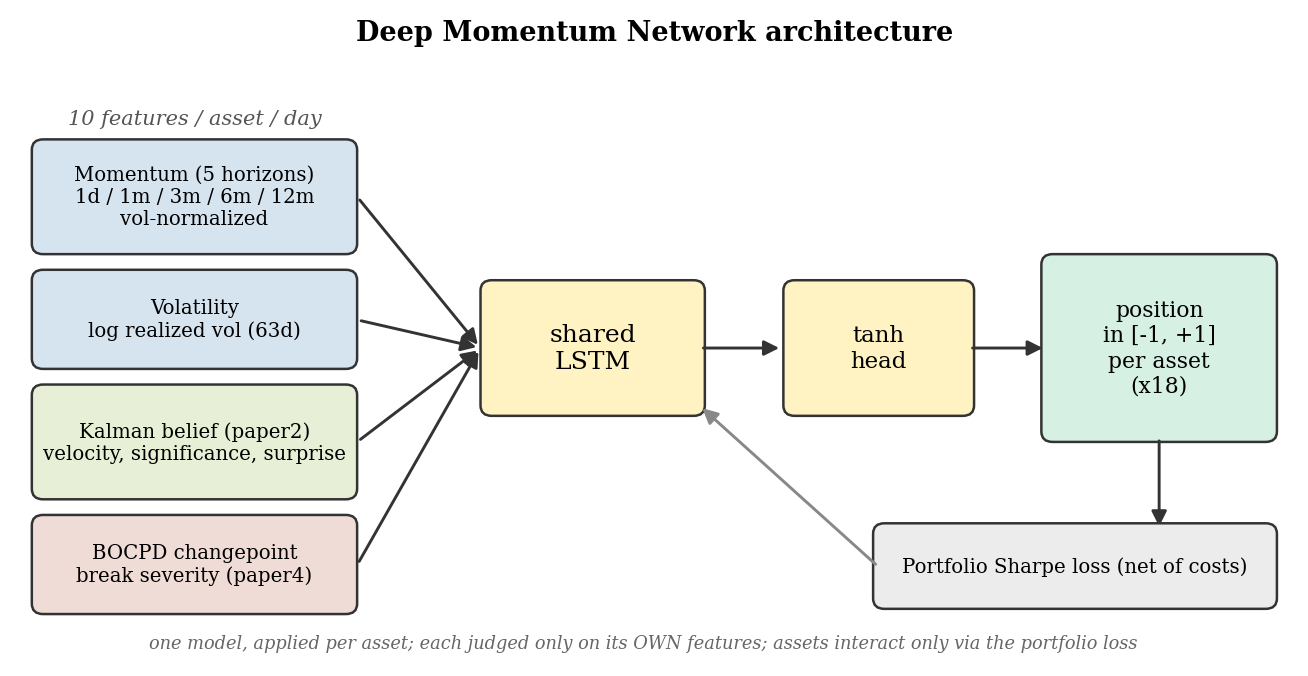
\includegraphics[width=.72\linewidth]{fig_architecture.png}
\caption{Για κάθε προϊόν, δέκα πληροφορίες ανά ημέρα τροφοδοτούν ένα LSTM· η έξοδος περνάει από μια
$\tanh$ και γίνεται θέση από $-1$ (πλήρης πώληση) έως $+1$ (πλήρης αγορά).}\end{figure}

\subsection{Είσοδος, δίκτυο, έξοδος}
Για \emph{κάθε} προϊόν ξεχωριστά, η είσοδος είναι μια ακολουθία από \textbf{δέκα χαρακτηριστικά} ανά
ημέρα: πέντε αποδόσεις διαφορετικού ορίζοντα κανονικοποιημένες με τη μεταβλητότητα, η ίδια η
μεταβλητότητα, τρεις δείκτες «πεποίθησης» από ένα φίλτρο Kalman, και ένα σήμα αλλαγής καθεστώτος
(BOCPD). Αυτή η ακολουθία περνάει από ένα \textbf{κοινό} LSTM, μετά από ένα γραμμικό στρώμα, και τέλος
από μια $\tanh$ που δίνει την τελική θέση στο $[-1,1]$:
\[
\text{θέση}_t \;=\; \tanh\big(\text{Linear}(h_t)\big)\in[-1,1].
\]
«Κοινό» σημαίνει ότι το \emph{ίδιο} δίκτυο εφαρμόζεται σε όλα τα προϊόντα --- μαθαίνει έναν γενικό
κανόνα «πώς μοιάζει μια αξιοποιήσιμη τάση», όχι ξεχωριστό κανόνα ανά μετοχή.

\key{Προσέξτε τι \emph{δεν} κάνει: δεν προσπαθεί να προβλέψει την αυριανή τιμή. Βγάζει \emph{κατευθείαν}
μια θέση. Δεν μας νοιάζει η ακριβής πρόβλεψη, μας νοιάζει η σωστή τοποθέτηση.}

\subsection{Η «απώλεια Sharpe»: ο έξυπνος στόχος}
Εδώ κρύβεται το πιο ενδιαφέρον. Αντί να εκπαιδεύσουμε το δίκτυο να μαντεύει τιμές, το εκπαιδεύουμε να
μεγιστοποιεί απευθείας την \textbf{ποιότητα του κέρδους} ολόκληρου του χαρτοφυλακίου. Αν
$\text{θέσεις}$ είναι οι τοποθετήσεις και $\text{απόδ}$ οι επόμενες αποδόσεις, η ημερήσια απόδοση του
χαρτοφυλακίου (αφαιρώντας ένα κόστος για τις αλλαγές θέσης, τον \emph{τζίρο}) είναι ένα διάνυσμα
$\text{port}$, και η συνάρτηση κόστους είναι το \textbf{αρνητικό} του Sharpe:
\[
\text{Loss} \;=\; -\,\frac{\text{μέσος}(\text{port})}{\text{τυπ.\ απόκλιση}(\text{port})}.
\]
Ελαχιστοποιώντας αυτό, μεγιστοποιούμε τον λόγο «κέρδος προς ρίσκο». Επειδή το $\text{port}$ είναι η
απόδοση \emph{όλου} του καλαθιού μαζί, η \textbf{διαφοροποίηση μπαίνει μέσα στον ίδιο τον στόχο}: το
δίκτυο ανταμείβεται όταν οι θέσεις του σε διαφορετικά προϊόντα αλληλοσυμπληρώνονται και τιμωρείται όταν
στοιβάζουν το ίδιο ρίσκο. Το κόστος τζίρου το αποτρέπει από νευρικές, ακριβές αλλαγές.

\subsection{Τίμια εκπαίδευση: χωρίς «κλεψιά»}
Ένα μοντέλο που έχει δει το μέλλον μοιάζει ιδιοφυές --- και είναι άχρηστο. Γι' αυτό εκπαιδεύουμε με
\textbf{φωλιασμένη διαδοχική επικύρωση} (nested walk-forward): το δίκτυο μαθαίνει αποκλειστικά από το
παρελθόν, διαλέγει τις ρυθμίσεις του (μέγεθος, κανονικοποίηση) σε ένα ενδιάμεσο κομμάτι επικύρωσης που
\emph{δεν} είναι το τεστ, και αξιολογείται μόνο σε μελλοντικά δεδομένα που δεν έχει αγγίξει. Προσθέτουμε
και τεχνικές σταθερότητας, όπως το «ψαλίδισμα» των κλίσεων ώστε η εκπαίδευση να μην εκτροχιάζεται.

\warnb{Χωρίς αυτή την πειθαρχία, οποιοδήποτε δίκτυο δείχνει εντυπωσιακά αποτελέσματα στο χαρτί που
\emph{εξαφανίζονται} στην πραγματικότητα. Η τιμιότητα της αξιολόγησης είναι πιο σημαντική από την
πολυπλοκότητα του μοντέλου.}

\subsection{Πώς δένει με τα υπόλοιπα}
Τα δέκα χαρακτηριστικά δεν είναι ακατέργαστες τιμές: είναι ήδη «καταστάσεις πεποίθησης» από το φίλτρο
Kalman και τον ανιχνευτή αλλαγής BOCPD. Έτσι το LSTM δεν ξεκινάει από το μηδέν --- παίρνει ήδη
επεξεργασμένες ενδείξεις τάσης και ρίσκου, και μαθαίνει πώς να τις μετατρέπει σε θέση. Στην πράξη αυτό
το ML μοντέλο ξεπερνά τον σταθερό κανόνα σε ποιότητα κέρδους, με μετρημένο αλλά υπαρκτό πλεονέκτημα.

\section*{Τι να κρατήσετε}
\begin{itemize}[nosep,leftmargin=1.4em]
\item Ένας \textbf{νευρώνας} ζυγίζει εισόδους και περνάει το άθροισμα από μια καμπύλη· ένα \textbf{δίκτυο} είναι πολλοί νευρώνες σε στρώματα.
\item Η \textbf{μάθηση} είναι κατάβαση σε ένα τοπίο κόστους, με τις κλίσεις να υπολογίζονται από το backpropagation.
\item Το \textbf{LSTM} προσθέτει ελεγχόμενη μνήμη με τρεις πύλες, ώστε να θυμάται τάσεις και να τις ξεχνάει όταν αλλάζει το καθεστώς.
\item Στη \textbf{δική μας} περίπτωση, ένα κοινό LSTM μετατρέπει δέκα belief-state χαρακτηριστικά σε θέση $[-1,1]$, εκπαιδευμένο να μεγιστοποιεί τον Sharpe όλου του χαρτοφυλακίου, με τίμια διαδοχική επικύρωση.
\end{itemize}

\vfill
\noindent\rule{\linewidth}{0.4pt}\\[2pt]
{\small QUANTIQ / AGEL AI. Εκπαιδευτικό συνοδευτικό της εργασίας \emph{«From Dead Cross-Sectional
Momentum to Belief-State Deep Time-Series Momentum»} (Drakos 2026).}

\end{document}
